\documentclass{article}

\usepackage[utf8]{inputenc} 
\usepackage[russian]{babel}

\usepackage{listings}
\usepackage{float}
\usepackage{amsmath}
\usepackage{breqn}
% allow utf-8 input
\usepackage{url}            % simple URL typesetting
\usepackage{booktabs}       % professional-quality tables
\usepackage{amsfonts}       % blackboard math symbols
\usepackage{subcaption}
\usepackage[labelformat=parens,labelsep=quad,skip=3pt]{caption}
\usepackage{graphicx}
\usepackage{color}

\usepackage{mathtools}

\usepackage{geometry} % Меняем поля страницы
\geometry{left=2cm}% левое поле
\geometry{right=2cm}% правое поле
\geometry{top=3cm}% верхнее поле
\geometry{bottom=2cm}% нижнее поле

\newtheorem{theorem}{Теорема}
\newtheorem{definition}{Опредление}
\newcommand\scalemath[2]{\scalebox{#1}{\mbox{\ensuremath{\displaystyle #2}}}}

\addto\captionsrussian{\def\refname{Список используемой литературы}}

\newcounter{totreferences}

\pretocmd{\bibitem}{\addtocounter{totreferences}{1}}{}{}


\definecolor{deepblue}{rgb}{0,0,0.5}
\definecolor{deepred}{rgb}{0.6,0,0}
\definecolor{deepgreen}{rgb}{0,0.5,0}

\DeclareFixedFont{\ttb}{T1}{txtt}{bx}{n}{12} % for bold
\DeclareFixedFont{\ttm}{T1}{txtt}{m}{n}{12} 

\lstset{
language=Python,
basicstyle=\ttm,
otherkeywords={self},             % Add keywords here
keywordstyle=\ttb\color{deepblue},
emph={MyClass,__init__},          % Custom highlighting
emphstyle=\ttb\color{deepred},    % Custom highlighting style
stringstyle=\color{deepgreen},
frame=tb,                         % Any extra options here
showstringspaces=false            % 
}

\title{Заголовок}

\begin{document}

\tableofcontents

\newpage

\section{Введение}

Целью данного проекта является расчет некоторых параметров открытого планарного диэлектрического волновода. Проект является командным и планируется, что каждый из членов команды внесет свой собственный вклад в решение.В начале проекта я взял на себя управленческую роль. Так что моей целью было получить навыки организации команды, контролю вектора развития проекта, а так же структурированию идей и отбрасываню
не нужных. Это важно, поскольку выполнение современных исследованиний и разработок в одиночку крайне затруднительно. Необходимо уметь работать в условия нехватки таких ресурсов, как: время, деньги, компетенция, тех. обеспечение. Ещё одной главной целью являлось получение навыков в моделировании физико технических явлений, которая в свою очередь включало в себя работу с пакетами символьных вычислений. Так нашем проекте мы используем Wolfram Mathematica и библиотеку символьных вычислений SymPy для языка Python.
\newpage

\section{Теоретическая часть}

Линза Люнеберга — линза, в которой показатель преломления не является постоянным, а изменяется по некоторому закону в зависимости от расстояния от центра в сферических или от оси в цилиндрических линзах. Обычно закон изменения показателя преломления подбирается таким образом, чтобы при прохождении линзы параллельные лучи фокусировались в одной точке на поверхности линзы, а испущенные точечным источником на поверхности — формировали параллельный пучок.

Подобная конструкция линз была впервые предложена немецким/американским математиком Рудольфом Люнебергом.\\[10pt]

\begin{figure}[H]
    \centering
    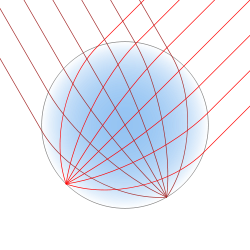
\includegraphics[width=120]{image3.png}
    \caption{}
    \label{tok_per_tweet}
\end{figure}

Линзы Люнеберга широко используются в СВЧ-технике. Одним из таких использований является создание сильно отражающих радиоволны объектов. В частности, линзы Люнеберга используются в ракетах-мишенях для имитации эффективной площади рассеяния реальных целей с бо́льшими размерами (например, боевых самолётов].

Использованию подобных линз в оптической технике препятствуют технические сложности изготовления линз с переменным показателем преломления, что определяет их высокую стоимость. Иногда для упрощения технологии производства подобные линзы собирают из дискретных элементов — небольших кубиков с различными показателями преломления.\\[10pt]

Линза Люнеберга долгое время оставалась не более чем математическим курьёзом, пока в начале 1960-х годов не была использована в качестве формирователя луча в американском радаре AN/SPG-59.

Радар AN/SPG-59 был одним из первых в мире радаров с фазированной антенной решёткой (ФАР). В отличие от современных радаров с ФАР, где пространственная картина луча формируется с помощью управляемых фазовращателей, в радаре AN/SPG-59 использовалась линза Люнеберга, расположенная в надстройке корабля. Выбор этой технологии был обусловлен отсутствием в 1960-х годах компактных и надёжных фазовращателей C-диапазона.

На поверхности линзы располагалось несколько тысяч приёмных и передающих элементов. Когда один из передающих элементов формировал на поверхности линзы сферическую радиоволну, линза преобразовывала её в волну с плоскопараллельными фронтами, фазовая картина которой снималась приёмными элементами и транслировалась на сферический излучатель, расположенный на вершине колоколообразной надстройки. Таким образом, сферический излучатель формировал в пространстве луч, направление которого соответствовало положению на линзе излучающего элемента.

\newpage

\section{Постановка задач}
В ТОВЛ Люнеберга распространение излучения описывается уравнениями Максвелла.

\begin{figure}[H]
    \centering
    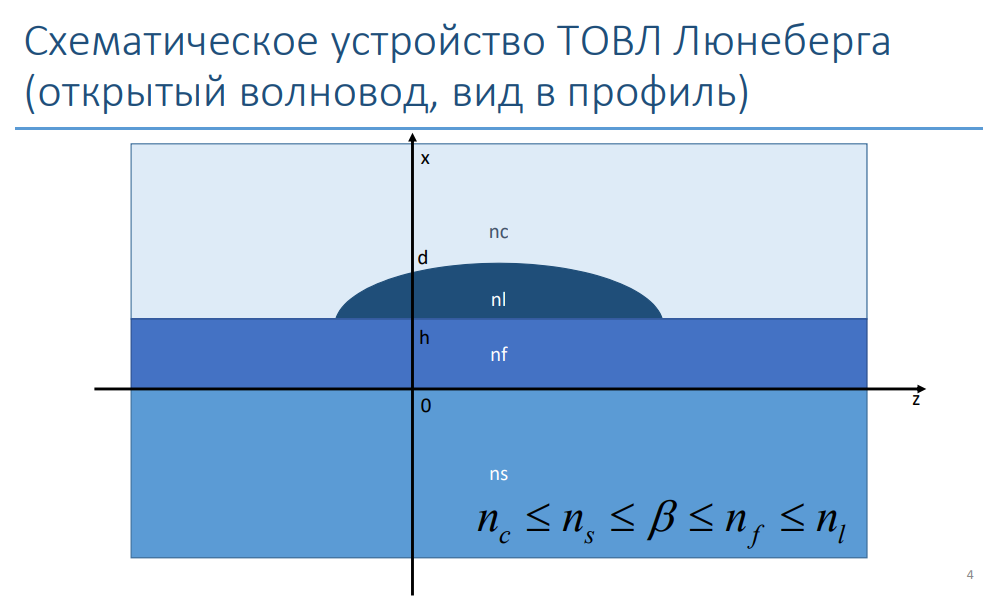
\includegraphics[width=\linewidth]{image2.png}
    \caption{Схематический вид ТОВЛ Люнеберга}
    \label{luneberg}
\end{figure}

\begin{definition}
{\bf Уравнения Максвелла} — система уравнений в дифференциальной или интегральной форме, описывающих электромагнитное поле и его связь с электрическими зарядами и токами в вакууме и сплошных средах.
\end{definition}

В нашей работе мы будем рассматривать трехслойник, который отличается от ТОВЛ Люнеберга, представленной на Рис. (2), отсутствием слоя $l$. На рисунке: $n_\tau, \tau = s, f, c$ - оптический показатель преломления в каждом соотв. слое.


\subsection{Формулировка Уравнений Максвелла}
В отсутствии внешних токов данные уравнения записываются в следющей форме\cite{luneberg2010}:
$$rot \vec{E} = - \frac{\mu}{c} \cdot \frac{\partial \vec{H}}{\partial t}$$
$$rot \vec{H} = \frac{\varepsilon}{c}\cdot\frac{\partial \vec{E}}{\partial t}$$

Где $\vec{E}$ - напряженность электрического поля, а $\vec{H}$ - напряженность магнитного поля. $c$ - скорость света в вакууме.

\par Общие решения уравнений максвелла являются полями мод плавно-нерегулярного волновода в адиабатическом приближении. Они имеют следующий вид:

$$\vec{E}(x, y, z, t) = \vec{E}(x, y, z) \cdot \frac{exp(i \omega t - i \phi(y, z)}{\sqrt{\beta(y, z)}}$$

$$\vec{H}(x, y, z, t) = \vec{H}(x, y, z) \cdot \frac{exp(i \omega t - i \phi(y, z)}{\sqrt{\beta(y, z)}}$$

где, $\beta(y, z) = \frac{1}{k_0} \sqrt{(\frac{\partial \phi}{\partial y})^2 + (\frac{\partial \phi}{\partial z})^2}$ - коэффициент фазового замедления.

Для данных полей справедливы следующие граничные условия:
\begin{itemize}
    \item Общие для TE,TM-мод:
    $$\vec{E}_\tau |_{x - 0} = \vec{E}_\tau |_{x + 0}, \vec{H}_\tau |_{x - o} = \vec{H}_\tau|_{x + 0} \eqno(a)$$
    \item Для TE-мод:
    $$\vec{H}_z|_{h-0} = \vec{H}_z|_{h+0}, \vec{E}_y|_{h-0} = \vec{E}_y|_{h + 0} \eqno(b)$$
    \item Для TM-мод:
    $$\vec{E}_z|_{h-0} = \vec{E}_z|_{h+0}, \vec{H}_y|_{h-0} = \vec{H}_y|_{h + 0} \eqno(c)$$
    \item Условие на бесконечности:
    $$|\vec{E}_\tau|_{x \to \pm \infty} < +\infty, |\vec{H}_\tau|_{x \to \pm\infty} < + \infty \eqno(d)$$
\end{itemize}

Где: $k_0 = \frac{2\pi}{\lambda} = \frac{\omega}{c}$ - модуль волнового вектора. $\lambda$ - длина волны света.
\subsection{Представление в виде СЛАУ}
В нулевом приближении асимптотического метода волновые уравнения для мод в каждом слое принимают следующий вид\cite{sevas2013}:

$$\frac{d^{2}E_{z}}{dx^{2}}+k_{0}^{2}\left(\varepsilon _{j}\mu_{j}-\beta ^{2}  \right)E_{z}=0 \eqno(1)$$

$$\frac{d^{2}H_{z}}{dx^{2}}+k_{0}^{2}\left(\varepsilon _{j}\mu _{j}-\beta ^{2} \right)H_{z}=0\eqno(2)$$

$$E_{y}=\frac{1}{k_{0}^{2}\left(\varepsilon \mu -\beta_{z}^{2} \right)}\left(\iota k_{0}\mu \frac{dH_{z}}{dx}\right)\eqno(3)$$

$$H_{y}=\frac{1}{k_{0}^{2}\left(\varepsilon \mu -\beta_{z}^{2} \right)}\left(-\iota k_{0}\varepsilon \frac{dE_{z}}{dx}  \right)\eqno(4)$$

{\bf Рассмотрим TE-моду.}\\
Введем обозначения:
$$
\gamma_\tau = k_0 \cdot \sqrt{\beta^2 - n_\tau^2}, \tau = s, f, c
$$
$$
\chi_\tau = k_0 \cdot \sqrt{n_\tau^2 - \beta^2}, \tau = s, f, c
$$
Для трехслойного волновода\cite{sevas_disser}, на границе слоев s и f ($x = a_1$) выполняются тангенциальные граничные условия (с), поскольку для ТЕ-моды $H_y == 0, E_y == 0$. Следовательно:
$$
\begin{cases}
H_z^s(a_1) = H_z^f(a_1) \Leftrightarrow 
C_{se2} exp(\gamma_s \cdot a_1) = C_{fe1}(i\chi_f \cdot a_1) + C_{fe2}(-i \chi_f \cdot a_1)\\
E_y^s(a1) = E_y^f(a1) \Leftrightarrow
\frac{ik_0}{\gamma_s} C_{se2} exp(\gamma_s \cdot a_1) = \frac{k_0}{\chi_f} \left ( C_{fe1}exp(i \chi_f \cdot a_1) + C_{fe2} exp(-i \chi_f \cdot a_1)\right )
\end{cases} \eqno(e)
$$
Соответственно, на границе слоев f и с ($x = a_2$):
$$
\begin{cases}
H_z^c(a_2) = H_z^f(a_2) \Leftrightarrow
C_{ce1} exp(-\gamma_c \cdot a_2) = C_{fe1}(i\chi_f \cdot a_2) + C_{fe2}(-i \chi_f \cdot a_2) \\
E_y^c(a_2) = E_y^f(a_2) \Leftrightarrow
-\frac{ik_0}{\gamma_c} C_{ce1} exp(-\gamma_c a_2) = \frac{k_0}{\chi_f} \left ( C_{fe1}exp(i \chi_f \cdot a_2) + C_{fe2} exp(-i \chi_f \cdot a_2)\right )
\end{cases} \eqno(f)
$$
Соотношения (e-f) образуют однородную СЛАУ для четерех неопределенных амплитудных коэффициентов $C_{ce1}, C_{fe1}, C_{fe2}, C_{se2}$. В матричном виде система выглядит следующим образом:
$$
\mathcal{M}_{TE}(\beta) \cdot A_{TE} = 0 \eqno(5)
$$ 
Где $A_{TE}$ - вектор $\{C_{ce1}, C_{fe1}, C_{fe2}, C_{se2}\}$. Система (5) разрешима при условии:
$$
det(\mathcal{M}_{TE}(\beta)) = 0
$$

Аналогично, для ТМ-моды выполняются условия (b), поскольку для TM-мод $H_z == 0, E_y == 0$. СЛАУ для неопределенных амплитудных коэффициентов $C_{ch1}, C_{fh1}, C_{fh2}, C_{sh2}$ имеет вид:
$$\mathcal{M}_{TM}(\beta) \cdot A_{TM} = 0 \eqno(6)$$
Где $A_{TM} = \{ C_{ch1}, C_{fh1}, C_{fh2}, C_{sh2} \}$. СЛАУ (6) так-же разрешима при условии: 
$$
det(\mathcal{M}_{TM}(\beta)) = 0
$$

\subsection{Формулировка задач}

В итоге необходимо решить следующие задачи:
\begin{enumerate}
    \item Из решений уравнений (1-4) с учетом граничных условий и условия для существования нетривиального решения вывести зависимость коэффициента фазового замедления $\beta$ от d при $det\left [ \mathcal{M}(x, \beta)\right ] = 0$.
    \item Получить значения неизвестных амплитудных коэффициентов $C_1, \ldots, C_n$ . Используя их, построить поле для любого из компонентов решения.
\end{enumerate}

\newpage

\section{Ход решения}

Ход решения поставленных задач состоит из следующих этапов:
\begin{enumerate}
    \item Нахождение компонент $E_z, H_z$ в общем виде путем решения уравнений (1), (2)
    \item Нахождение компонент $E_y, H_y$ в общем виде из формул (3), (4).
    \item Подстановка компонент в граничные условия, разделение полученных уравнений на TE,TM-моды (независимые группы уравнений).
    \item Приведение СЛАУ к матричному виду: $\mathcal{M}(\beta, d) \cdot A = 0$. 
    \item Нахождение зависимости $\beta$ от d при $\mathcal{M}(\beta, d) \cdot A = 0$.
\end{enumerate}

Далее подробно опишем действия на каждом шаге. Все вычисления выполнялись с помощью библиотеки для символьных вычислений SymPy версии 1.4 для языка Python версии 3.7.

\subsection{Компоненты $E_z, H_z$}
Получим компоненты $E_z, H_z$ в общем виде путем нахождения ФСР (1), (2):

$$\operatorname{E_{z}}{\left (x \right )} = C_{e1} e^{- \frac{2 \pi x \sqrt{\beta^{2} - \epsilon_{s} \mu_{s}}}{\lambda}} + C_{e2} e^{\frac{2 \pi x \sqrt{\beta^{2} - \epsilon_{s} \mu_{s}}}{\lambda}} \eqno(5)$$
$$\operatorname{H_{z}}{\left (x \right )} = C_{h1} e^{- \frac{2 \pi x \sqrt{\beta^{2} - \epsilon_{s} \mu_{s}}}{\lambda}} + C_{h2} e^{\frac{2 \pi x \sqrt{\beta^{2} - \epsilon_{s} \mu_{s}}}{\lambda}} \eqno(6)$$

\subsection{Компоненты $E_z, H_z$}

Продифференцируем компоненты $E_z, H_z$, по $z$, и подставим результат в (3), (4) соответственно. Получим:
$$H_y=\frac{\lambda^{2} \left(- \frac{4 \pi^{2} \beta_{y} \beta_{z} \left(C_{ch1} e^{- \frac{2 \pi x \sqrt{\beta^{2} - \epsilon_{c} \mu_{c}}}{\lambda}} + C_{ch2} e^{\frac{2 \pi x \sqrt{\beta^{2} - \epsilon_{c} \mu_{c}}}{\lambda}}\right)}{\lambda^{2}} - \frac{2 i \pi \epsilon_{c} \left(- \frac{2 \pi C_{ce1} \sqrt{\beta^{2} - \epsilon_{c} \mu_{c}} e^{- \frac{2 \pi x \sqrt{\beta^{2} - \epsilon_{c} \mu_{c}}}{\lambda}}}{\lambda} + \frac{2 \pi C_{ce2} \sqrt{\beta^{2} - \epsilon_{c} \mu_{c}} e^{\frac{2 \pi x \sqrt{\beta^{2} - \epsilon_{c} \mu_{c}}}{\lambda}}}{\lambda}\right)}{\lambda}\right)}{4 \pi^{2} \left(- \beta_{z}^{2} + \epsilon_{c} \mu_{c}\right)}\eqno(7)$$

$$E_y=\frac{\lambda^{2} \left(\frac{4 \pi^{2} \beta_{y} \beta_{z} \left(C_{ce1} e^{- \frac{2 \pi x \sqrt{\beta^{2} - \epsilon_{c} \mu_{c}}}{\lambda}} + C_{ce2} e^{\frac{2 \pi x \sqrt{\beta^{2} - \epsilon_{c} \mu_{c}}}{\lambda}}\right)}{\lambda^{2}} + \frac{2 i \pi \mu_{c} \left(- \frac{2 \pi C_{ch1} \sqrt{\beta^{2} - \epsilon_{c} \mu_{c}} e^{- \frac{2 \pi x \sqrt{\beta^{2} - \epsilon_{c} \mu_{c}}}{\lambda}}}{\lambda} + \frac{2 \pi C_{ch2} \sqrt{\beta^{2} - \epsilon_{c} \mu_{c}} e^{\frac{2 \pi x \sqrt{\beta^{2} - \epsilon_{c} \mu_{c}}}{\lambda}}}{\lambda}\right)}{\lambda}\right)}{4 \pi^{2} \left(- \beta_{z}^{2} + \epsilon_{c} \mu_{c}\right)}\eqno(8)$$
(Для каждого слоя компоненты разные. Они отличаются значениями констант C. Поэтому далее каждая константа будет иметь дополнительный индекс - название слоя)

\subsection{Подстановка компонент в граничные условия, формирование СЛАУ, разделение полученных уравнений для TE,TM-мод.}
Имеем уравнения (5-8) в каждом слое (f, s, c) и граничные условия (a-d). Подставим уравнения (5-8) в граничные условия (a-d). Для граничных условий заметим, что они эквивалентны следующим уравнениям:
$$\begin{cases}
E_y^c = E_y^f\\
H_y^c = H_y^f\\
x = d
\end{cases} \eqno(9)$$
$$\begin{cases}
E_y^f = E_y^s \\
H_y^f = H_y^f\\
x = 0
\end{cases} \eqno(10)$$
$$\begin{cases}
E_z^c = E_z^f \\
H_z^c = H_z^f\\
x = d
\end{cases} \eqno(11)$$
$$\begin{cases}
E_z^f = E_z^s \\
H_z^f = H_z^s\\
x = 0
\end{cases} \eqno(12)$$
$$\begin{cases}
\lim_{x \to +\infty} E^c_z(x) = 0\\
\lim_{x \to +\infty} H^c_z(x) = 0
\end{cases} \eqno(13)$$
$$\begin{cases}
\lim_{x \to -\infty} E^s_z(x) = 0\\
\lim_{x \to -\infty} H^s_z(x) = 0
\end{cases} \eqno(14)$$
\par Компоненты $E_z, H_z$ имеют вид $C_1a + C_2b$. Для выполнения граничных условий на бесконечности (d), необходимо чтобы при $x \to \pm \infty$ компоненты $H_z, E_z$ в слое $с$ ($+\infty$) стремились к нулю. Но при $x \to \pm \infty$ значение $а \to \pm \0$, а значение $b \to \pm \infty$. Из решения предельного уравнения 0 = $C_1*0 + C_2*\infty$ получаем, что $C_2 = 0$ в слое $c$. Из аналогичных рассуждений следует что $C_1 = 0$ в слое $s$.    

Из уравнений систем (9)-(14), составляем СЛАУ. СЛАУ можно разделить на TE и TM моды в силу независимости уравнений. Они выглядят следующим образом (Для слоев с и s некоторые константы обнулены из рассуждений выше):
$$\begin{cases}
C_{fe1} + C_{fe2} - C_{se2} = 0\\
C_{fe1} \beta_{z}^{2} \epsilon_{f} \sqrt{- \beta^{2} + \epsilon_{f} \mu_{f}} - C_{fe1} \epsilon_{f} \epsilon_{s} \mu_{s} \sqrt{- \beta^{2} + \epsilon_{f} \mu_{f}} - C_{fe2} \beta_{z}^{2} \epsilon_{f} \sqrt{- \beta^{2} + \epsilon_{f} \mu_{f}} +\\~~~~~~
C_{fe2} \epsilon_{f} \epsilon_{s} \mu_{s} \sqrt{- \beta^{2} + \epsilon_{f} \mu_{f}} - i C_{se2} \beta_{z}^{2} \epsilon_{s} \sqrt{\beta^{2} - \epsilon_{s} \mu_{s}} + i C_{se2} \epsilon_{f} \epsilon_{s} \mu_{f} \sqrt{\beta^{2} - \epsilon_{s} \mu_{s}} = 0\\
C_{ce1} e^{- \frac{2 \pi d \sqrt{\beta^{2} - \epsilon_{c} \mu_{c}}}{\lambda}} - C_{fe1} e^{- \frac{2 i \pi d \sqrt{- \beta^{2} + \epsilon_{f} \mu_{f}}}{\lambda}} - C_{fe2} e^{\frac{2 i \pi d \sqrt{- \beta^{2} + \epsilon_{f} \mu_{f}}}{\lambda}} = 0\\
- 4 i \pi^{2} C_{ce1} \beta^{2} \epsilon_{c} \sqrt{\beta^{2} - \epsilon_{c} \mu_{c}} e^{- \frac{2 \pi d \sqrt{\beta^{2} - \epsilon_{c} \mu_{c}}}{\lambda}} + 4 i \pi^{2} C_{ce1} \epsilon_{c} \epsilon_{f} \mu_{f} \sqrt{\beta^{2} - \epsilon_{c} \mu_{c}} \\ ~~~~~~ e^{- \frac{2 \pi d \sqrt{\beta^{2} - \epsilon_{c} \mu_{c}}}{\lambda}} - 4 \pi^{2} C_{fe1} \beta^{2} \epsilon_{f} \sqrt{- \beta^{2} + \epsilon_{f} \mu_{f}} e^{- \frac{2 i \pi d \sqrt{- \beta^{2} + \epsilon_{f} \mu_{f}}}{\lambda}} + 4 \pi^{2} C_{fe1} \epsilon_{c} \epsilon_{f} \mu_{c} \sqrt{- \beta^{2} + \epsilon_{f} \mu_{f}} e^{- \frac{2 i \pi d \sqrt{- \beta^{2} + \epsilon_{f} \mu_{f}}}{\lambda}} + 4 \\~~~~~~\pi^{2} C_{fe2} \beta^{2} \epsilon_{f} \sqrt{- \beta^{2} + \epsilon_{f} \mu_{f}} e^{\frac{2 i \pi d \sqrt{- \beta^{2} + \epsilon_{f} \mu_{f}}}{\lambda}} - 4 \pi^{2} C_{fe2} \epsilon_{c} \epsilon_{f} \mu_{c} \sqrt{- \beta^{2} + \epsilon_{f} \mu_{f}} e^{\frac{2 i \pi d \sqrt{- \beta^{2} + \epsilon_{f} \mu_{f}}}{\lambda}} = 0
\end{cases}\eqno(TE)$$

$$\begin{cases}
C_{fh1} + C_{fh2} - C_{sh2} = 0\\
- C_{fh1} \beta_{z}^{2} \mu_{f} \sqrt{- \beta^{2} + \epsilon_{f} \mu_{f}} + C_{fh1} \epsilon_{s} \mu_{f} \mu_{s} \sqrt{- \beta^{2} + \epsilon_{f} \mu_{f}} + C_{fh2} \beta_{z}^{2} \mu_{f} \sqrt{- \beta^{2} + \epsilon_{f} \mu_{f}} - C_{fh2} \epsilon_{s} \mu_{f}\\ ~~~~~~ \mu_{s} \sqrt{- \beta^{2} + \epsilon_{f} \mu_{f}} + i C_{sh2} \beta_{z}^{2} \mu_{s} \sqrt{\beta^{2} - \epsilon_{s} \mu_{s}} - i C_{sh2} \epsilon_{f} \mu_{f} \mu_{s} \sqrt{\beta^{2} - \epsilon_{s} \mu_{s}} = 0\\
C_{ch1} e^{- \frac{2 \pi d \sqrt{\beta^{2} - \epsilon_{c} \mu_{c}}}{\lambda}} - C_{fh1} e^{- \frac{2 i \pi d \sqrt{- \beta^{2} + \epsilon_{f} \mu_{f}}}{\lambda}} - C_{fh2} e^{\frac{2 i \pi d \sqrt{- \beta^{2} + \epsilon_{f} \mu_{f}}}{\lambda}} = 0\\
4 i \pi^{2} C_{ch1} \beta^{2} \mu_{c} \sqrt{\beta^{2} - \epsilon_{c} \mu_{c}} e^{- \frac{2 \pi d \sqrt{\beta^{2} - \epsilon_{c} \mu_{c}}}{\lambda}} - 4 i \pi^{2} C_{ch1} \epsilon_{f} \mu_{c} \mu_{f} \sqrt{\beta^{2} - \epsilon_{c} \mu_{c}}\\~~~~~~ e^{- \frac{2 \pi d \sqrt{\beta^{2} - \epsilon_{c} \mu_{c}}}{\lambda}} + 4 \pi^{2} C_{fh1} \beta^{2} \mu_{f} \sqrt{- \beta^{2} + \epsilon_{f} \mu_{f}} e^{- \frac{2 i \pi d \sqrt{- \beta^{2} + \epsilon_{f} \mu_{f}}}{\lambda}} - 4 \pi^{2} C_{fh1} \epsilon_{c} \mu_{c} \mu_{f} \sqrt{- \beta^{2} + \epsilon_{f} \mu_{f}} e^{- \frac{2 i \pi d \sqrt{- \beta^{2} + \epsilon_{f} \mu_{f}}}{\lambda}} - 4 \pi^{2} C_{fh2} \\~~~~~~ \beta^{2} \mu_{f} \sqrt{- \beta^{2} + \epsilon_{f} \mu_{f}} e^{\frac{2 i \pi d \sqrt{- \beta^{2} + \epsilon_{f} \mu_{f}}}{\lambda}} + 4 \pi^{2} C_{fh2} \epsilon_{c} \mu_{c} \mu_{f} \sqrt{- \beta^{2} + \epsilon_{f} \mu_{f}} e^{\frac{2 i \pi d \sqrt{- \beta^{2} + \epsilon_{f} \mu_{f}}}{\lambda}} = 0
\end{cases} \eqno(TM) $$


\subsection{Приводим СЛАУ к матричному виду $\mathcal{M}(\beta, d) \cdot A = 0$}
Представим наши системы уранений в матричном виде $\mathcal{M}(x, \beta) \cdot A = 0$. Где вектор неизвестных $A$ - вектор констант (Для ТЕ моды этот вектор = {$C_{ce1}, C_{fe1}, C_{fe2}, C_{se2}$}, для ТМ моды = {$C_{ch1}, C_{fh1}, C_{fh2}, C_{sh2}$}). Это было реализованно с помощью метода linear\_eq\_to\_matrix().

\subsection{Ищем значения для $\beta$ при $det(\mathcal{M}(\beta, d)) = 0$ }

Имеем определители: $$D_{TE} = det(\mathcal{M}_{TE}), D_{TM} = det(\mathcal{M}_{TM})$$
Уравнения имеют нетривиальное решение при условии $D_{TE} * D_{TM} = 0$. Опишем в общем случае методику нахождения зависимости $\beta(d)$.
\par Опретелители $D_{TE}$ и $D_{TM}$ зависит от двух переменных $d, \beta$. Составим сетку значений $d$: $d_i \in (d_1, d_2, \ldots, d_n)$. Для каждого $d_i$ составим зависимость $D_{TE}(\beta), D_{TM}(\beta)$. Это нужно для того, чтобы найти значения $\beta$, при которых $D_{TE}(\beta)$=0. Поиск будем проводить следующим образом: \begin{enumerate}
    \item Возьмем квадрат модуля $D_{TM}(\beta)$, чтобы  $\forall \beta$~:~$|D_{TM}(\beta)|^2 \geq 0$ для того, чтобы избавиться от мнимой части определителя и для возможности использовать методы поиска минимума. Из этого следует, что если существует такая $\beta': |D_{TM}(\beta')|^2 = 0 $, то $ D_{TM}(\beta') = 0$. Аналогично для $D_{TE}(\beta)$.
    \item Далее найдем область глобального минимума: разобьем значения $\beta$ на сетку: $d$: $\beta_i \in (\beta_1, \beta_2, \ldots, \beta_n)$. Вычтем из каждого элемента предыдущий элемент сетки и запишем значения в новый список (Это будет список условных производных в точках сетки). Пройдемся по полученному списку и найдем две соседние точки, на которых значение меняет знак с минуса на плюс. Эти точки являются границами области локального минимума.   
    \item В этих областях для поиска  минимума используем метод Нелдер-Мида со штрафами за пределами области.
    \item Если определитель в найденном минимуме равен нулю с заданной точностью, сохраняем значение бетта в данной точке для зафиксированного d. 
\end{enumerate}

Решая такую задачу для каждого $d_i$ из сетки получаем набор пар $$B = \left( \{d_1 \to \beta_1\}, \{d_2 \to \beta_2\}, \ldots, \{d_n \to \beta_n\}  \right )$$

В результате проведенных вычислений получены следующие зависимости.

\begin{figure}[H]
    \centering
    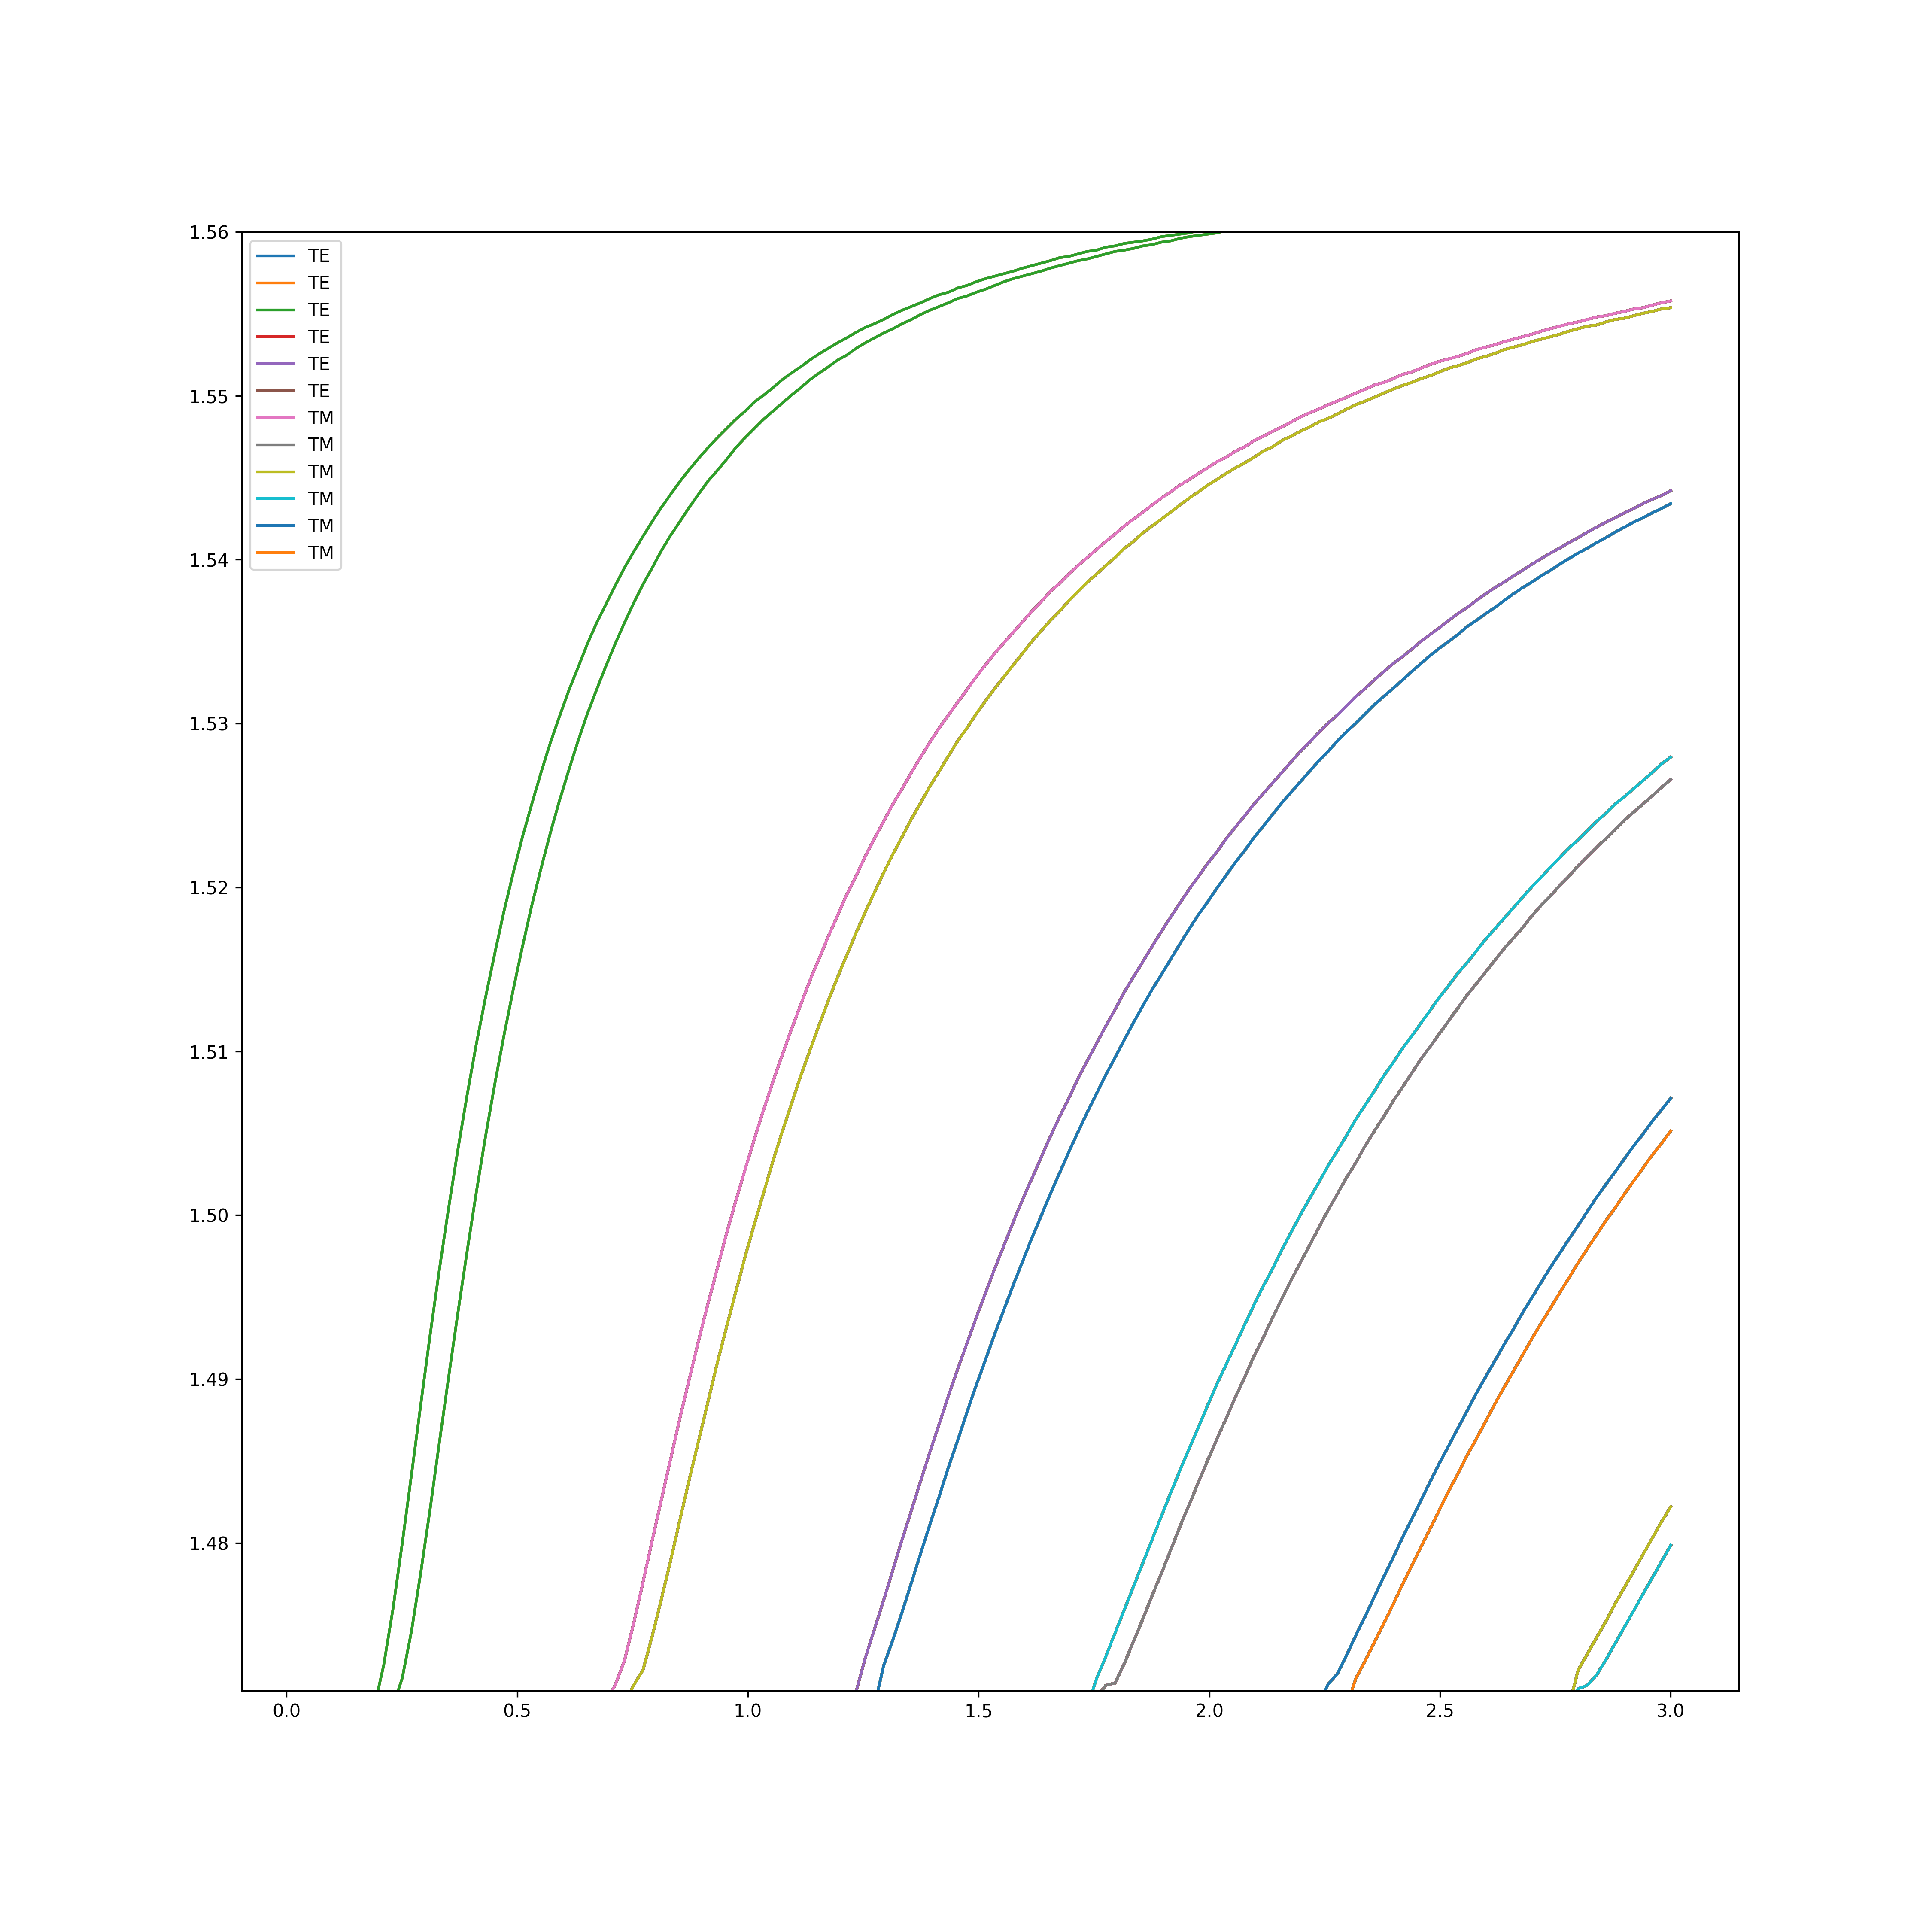
\includegraphics[width=\linewidth]{final.png}
    \caption{Графики $\beta$ от $z$ для мод TE, TM (в каждой паре графиков, одущих близко дргу к другу одна линия принадлежит зависимости в моде TE, другая - зависимости в моде TM)}
    \label{beta_d}
\end{figure}

Конфигурация вычислений:
\begin{itemize}
    \item Диапазон значений $\beta$: $(1.4695, 1.56505)$
    \item Диапазон значений $d$: $(0.01, 3)$
    \item Параметр точности вычислений $\epsilon$: $10e-6$
    \item Алгоритм минимизации: Nelder-Mead \cite{nelder1965simplex}.
\end{itemize}

Код приведен в приложении, см. стр 18.

\newpage

\section{Заключение}

По мере выполнение данной работы я выполнял различные задачи. Первичной моей работа был управленческая:
\begin{itemize}

\item организация встреч для обсуждения действий, нужно было подобрать такое время чтобы мы все смогли собраться на определенный период времени в одном месте
\item распределение работы между участниками проекта, чтобы все были заняты определенной работой и не было простоя в распределяемых задачах
\item настрой коллектива на работу, без нужного настроя коллектив быстро терял внимание и уходил в другие вопросы
\item проверка выполненной работы, по течению недели были некоторые задачи, которые тоже требовали контроля
\item заставлял задавать вопросы в общий чат, когда они возникали
Так же помимо этого я занимался некоторыми другими задачами:
\item перепроверил руками решение однородных дифференциальных уравнений второго порядка
\item помогал с написанием части кода в начале проекта, дальше помогал с поиском некоторых полезных функций
\item проверял встроенные методы для подсчёта констант
\end{itemize}
По мере проекта я приобрёл хорошие управленческие навыки, в том числе нашёл свои слабости в этом вопросе. Так же освежил свои знания по решению дифференциальных уравнений и линейной алгебре. Приобрёл навыки в решении физических задач.


\newpage

\addcontentsline{toc}{section}{Список используемой литературы}
\bibliographystyle{plain}
\bibliography{references.bib}

\newpage

\addcontentsline{toc}{section}{Приложения}
\section*{Приложения}
\subsection*{A - Исходный код}
\begin{lstlisting}[language=Python]

# coding: utf-8

# In[1]:


import math
from scipy.optimize import minimize, newton
import copy
import mpmath

from joblib import Parallel, delayed

import sympy
from sympy import Function, dsolve, Eq,
    Derivative, sin, cos, symbols, pi, I
from sympy.abc import x, y, z

from numba import jit
get_ipython().run_line_magic('matplotlib', 'inline')
sympy.init_session(use_latex=True)

epsilon = symbols("epsilon")
mu = symbols("mu")
lambda_ = symbols("lambda") ## длинна волны света 0.55
k0 = (pi * 2) / lambda_ 

phi = Function("phi")
betta = symbols("beta", real=True)  # Проницаемость среды
betta_y = symbols("beta_y")
betta_z = symbols("beta_z")

betta_y_test = Derivative(phi(y), y) 
betta_z_test = Derivative(phi(z), y)  

E_z = Function('E_z') 
H_z = Function('H_z')

epsilon_s = symbols("epsilon_s") 
mu_s = symbols("mu_s")

Ce_s1 = symbols("C_se1") 
Ce_s2 = symbols("C_se2")  
Ch_s1 = symbols("C_sh1") 
Ch_s2 = symbols("C_sh2") 

eq_s_ez = Derivative(E_z(x), x, x) +
    (k0**2)*(epsilon_s*mu_s - betta**2)*E_z(x)
eq_s_hz = Derivative(H_z(x), x, x) +
    (k0**2)*(epsilon_s*mu_s - betta**2)*H_z(x)

eq_s_ez_sloved = dsolve(eq_s_ez)
eq_s_hz_sloved = dsolve(eq_s_hz)

eq_s_ez_sloved = eq_s_ez_sloved.subs([["C1", Ce_s1], ["C2", Ce_s2]])
eq_s_hz_sloved = eq_s_hz_sloved.subs([["C1", Ch_s1], ["C2", Ch_s2]])


# In[33]:


epsilon_f = symbols("epsilon_f") # Электрическая проницаемость
mu_f = symbols("mu_f")  # Магнитная проницаемостьт

Ce_f1 = symbols("C_fe1") 
Ce_f2 = symbols("C_fe2")  
Ch_f1 = symbols("C_fh1") 
Ch_f2 = symbols("C_fh2")  

eq_f_ez = Derivative(E_z(x), x, x) +
    (k0**2)*(epsilon_f*mu_f - betta**2)*E_z(x)
eq_f_hz = Derivative(H_z(x), x, x) +
    (k0**2)*(epsilon_f*mu_f - betta**2)*H_z(x)

eq_f_ez_sloved = dsolve(eq_f_ez)
eq_f_hz_sloved = dsolve(eq_f_hz)

eq_f_ez_sloved = eq_f_ez_sloved.subs([["C1", Ce_f1], ["C2", Ce_f2]])
eq_f_hz_sloved = eq_f_hz_sloved.subs([["C1", Ch_f1], ["C2", Ch_f2]])

eq_f_hz_sloved = eq_f_hz_sloved.subs({
    betta:betta*I,
    epsilon_f:-epsilon_f,
    pi:pi*I
})

eq_f_ez_sloved = eq_f_ez_sloved.subs({
    betta:betta*I,
    epsilon_f:-epsilon_f,
    pi:pi*I
})

epsilon_c = symbols("epsilon_c") # Электрическая проницаемость
mu_c = symbols("mu_c")  # Магнитная проницаемостьт

Ce_c1 = symbols("C_ce1") 
Ce_c2 = symbols("C_ce2")  
Ch_c1 = symbols("C_ch1") 
Ch_c2 = symbols("C_ch2")  

eq_c_ez = Derivative(E_z(x), x, x) +
    (k0**2)*(epsilon_c*mu_c - betta**2)*E_z(x)
eq_c_hz = Derivative(H_z(x), x, x) +
    (k0**2)*(epsilon_c*mu_c - betta**2)*H_z(x)

eq_c_ez_sloved = dsolve(eq_c_ez)
eq_c_hz_sloved = dsolve(eq_c_hz)

eq_c_ez_sloved = eq_c_ez_sloved.subs([["C1", Ce_c1], ["C2", Ce_c2]])
eq_c_hz_sloved = eq_c_hz_sloved.subs([["C1", Ch_c1], ["C2", Ch_c2]])


left_part = (1 / ((k0**2)*(epsilon_c*mu_c - betta_z**2)))
E_y_c = left_part*(I*k0*mu_c*
    Derivative(H_z(x), x)+(k0**2)*betta_y*betta_z*E_z(x))
H_y_c = left_part*(-(k0**2)*
    betta_y*betta_z*H_z(x)-I*k0*epsilon_c*Derivative(E_z(x), x))
#f
left_part = (1 / ((k0**2)*
    (epsilon_f*mu_f - betta_z**2)))
E_y_f = left_part*(I*k0*mu_f*
    Derivative(H_z(x), x)+(k0**2)*betta_y*betta_z*E_z(x))
H_y_f = left_part*(-(k0**2)*
    betta_y*betta_z*H_z(x)-I*k0*epsilon_f*Derivative(E_z(x), x))
#s
left_part = (1 / ((k0**2)*
    (epsilon_s*mu_s - betta_z**2)))
E_y_s = left_part*(I*k0*mu_s*
    Derivative(H_z(x), x)+(k0**2)*betta_y*betta_z*E_z(x))
H_y_s = left_part*(-(k0**2)*
    betta_y*betta_z*H_z(x)-I*k0*epsilon_s*Derivative(E_z(x), x))

eq_c_hz_diff = diff(eq_c_hz_sloved.rhs,x)
eq_s_hz_diff = diff(eq_s_hz_sloved.rhs,x)
eq_f_hz_diff = diff(eq_f_hz_sloved.rhs,x)
eq_c_ez_diff = diff(eq_c_ez_sloved.rhs,x)
eq_s_ez_diff = diff(eq_s_ez_sloved.rhs,x)
eq_f_ez_diff = diff(eq_f_ez_sloved.rhs,x)

H_y_c = H_y_c.subs({
    H_z(x) : eq_c_hz_sloved.rhs,
    Derivative(E_z(x), x) : eq_c_ez_diff,
})

H_y_f = H_y_f.subs({
    H_z(x) : eq_f_hz_sloved.rhs,
    Derivative(E_z(x), x) : eq_f_ez_diff,
})

H_y_s = H_y_s.subs({
    H_z(x) : eq_s_hz_sloved.rhs,
    Derivative(E_z(x), x) : eq_s_ez_diff,
})

E_y_c = E_y_c.subs({
    E_z(x) : eq_c_ez_sloved.rhs,
    Derivative(H_z(x), x) : eq_c_hz_diff,
})

E_y_f = E_y_f.subs({
    E_z(x) : eq_f_ez_sloved.rhs,
    Derivative(H_z(x), x) : eq_f_hz_diff,
})

E_y_s = E_y_s.subs({
    E_z(x) : eq_s_ez_sloved.rhs,
    Derivative(H_z(x), x) : eq_s_hz_diff,
})

fez_sloved = eq_f_ez_sloved
fhz_sloved = eq_f_ez_sloved

Ez_cf = Equality(eq_c_ez_sloved.rhs - eq_f_ez_sloved.rhs, 0)
Ez_fs = Equality(eq_f_ez_sloved.rhs - eq_s_ez_sloved.rhs, 0)

Hz_cf = Equality(eq_c_hz_sloved.rhs - eq_f_hz_sloved.rhs, 0)
Hz_fs = Equality(eq_f_hz_sloved.rhs - eq_s_hz_sloved.rhs, 0)

Ey_cf = Equality(E_y_c - E_y_f, 0)
Ey_fs = Equality(E_y_f - E_y_s, 0)

Hy_cf = Equality(H_y_c - H_y_f, 0)
Hy_fs = Equality(H_y_f - H_y_s, 0)

Ez_fs = Ez_fs.subs({
    'x': 0, 'beta': betta_z,
    'C_ce2': 0, 'C_ch2': 0,
    'C_se1': 0, 'C_sh1': 0
})
Hz_fs = Hz_fs.subs({
    'x': 0, 'beta': betta_z,
    'C_ce2': 0, 'C_ch2': 0,
    'C_se1': 0, 'C_sh1': 0
})
Ey_fs = Ey_fs.subs({
    'x': 0, 'beta_y': 0,
    'beta': betta_z, 'C_ce2': 0,
    'C_ch2': 0, 'C_se1': 0, 'C_sh1': 0
})
Hy_fs = Hy_fs.subs({
    'x': 0, 'beta_y': 0,
    'beta': betta_z, 'C_ce2': 0,
    'C_ch2': 0, 'C_se1': 0, 'C_sh1': 0
})

d = symbols("d")

Ey_fs_ = Equality(Ey_fs.lhs * 
    (epsilon_s*mu_s - betta_z**2) * 
    (((2*pi)*(epsilon_f*mu_f - betta_z**2))), 0)
.simplify()
Hy_fs_ = Equality(Hy_fs.lhs * 
    (epsilon_s*mu_s - betta_z**2) * 
    (((2*pi)*(epsilon_f*mu_f - betta_z**2))), 0)
.simplify()
Ey_cf_ = Equality(Ey_cf.lhs * 
    (epsilon_c*mu_c - betta_z**2) * 
    (((2*pi)*(2*pi)*(epsilon_f*mu_f - betta_z**2))), 0)
.simplify()
Hy_cf_ = Equality(Hy_cf.lhs * 
    (epsilon_c*mu_c - betta_z**2) * 
    (((2*pi)*(2*pi)*(epsilon_f*mu_f - betta_z**2))), 0)
.simplify()

Ey_fs_new = Equality(Ey_fs_.lhs * 1/(2*pi), 0)
Hy_fs_new = Equality(Hy_fs_.lhs * 1/(2*pi), 0)

Hy_fs_new.expand()

Ez_cf_kek = Ez_cf.subs({
    betta_y : 0,
    Ce_c2 : 0,
    x : d
})
Ez_cf_kek
Hz_cf_kek = Hz_cf.subs({
    betta_y : 0,
    Ch_c2 : 0,
    x : d
})

Hy_cf_kek = Hy_cf_.subs({
    betta_y : 0,
    Ce_c2 : 0,
    betta_z : betta,
    x : d
})
Hy_cf_kek_expand = Hy_cf_kek.expand()
Ey_cf_kek = Ey_cf_.subs({
    betta_y : 0,
    Ch_c2 : 0,
    betta_z : betta,
    x : d
})
Ey_cf_kek_expand = Ey_cf_kek.expand()

L1_kek = sympy.linear_eq_to_matrix(
    [Ez_fs, Hy_fs_new.expand(), Ez_cf_kek, Hy_cf_kek_expand],
    Ce_c1, Ce_f1, Ce_f2, Ce_s2
)[0]
L2_kek = sympy.linear_eq_to_matrix(
    [Hz_fs, Ey_fs_new.expand(), Hz_cf_kek, Ey_cf_kek_expand],
    Ch_c1, Ch_f1, Ch_f2, Ch_s2
)[0]

L1_kek = L1_kek.subs({
    mu_c : 1,
    mu_f : 1,
    mu_s : 1,
    lambda_ : 0.55,
    #h: 2*lambda_,
    betta_z: betta,
    epsilon_c : 1,
    epsilon_f : 1.565 ** 2,
    epsilon_s : 1.47 ** 2
})

L2_kek = L2_kek.subs({
    mu_c : 1,
    mu_f : 1,
    mu_s : 1,
    lambda_ : 0.55,
    #h: 2*lambda_,
    betta_z: betta,
    epsilon_c : 1,
    epsilon_f : 1.565 ** 2,
    epsilon_s : 1.47 ** 2
})

omg = L1_kek.det()
omg2 = L2_kek.det()

class DBettaAdapter:
    def __init__(self, left, right, determinant, d_):
        self.init_right_bound = right
        self.init_left_bound = left
        self.raw_deterninant = determinant
        self.set_d(d_)
        self.factor = 1
        self.epsilon = 1e-6
        self.min = []
    
    def set_d(self, d_):
        self.determinant = self.raw_deterninant.subs({"d":d_})
        self.d = d_

    def set_bounds(self, left, right):
        self.right_bound = right
        self.left_bound = left
    
    def func(self, b):
        b = b[0]
        eval_ = self.determinant.evalf(subs={betta:b})
        if b < self.left_bound or b > self.right_bound:
            return 1000
        else:
            ans = mpmath.power(Abs(eval_), 2)
        return ans * self.factor

    def opt(self):
        mid = (self.right_bound - self.left_bound)/2 + self.left_bound
        res = minimize(self.func, [mid], method ="BFGS")#
        return res
    
    def draw_plot(self, num_points=100):
        #for i in arr:
        #    res_.append(self.func([i]))
        arr, step, res_ = self.eval_array(num_points)
        
        plt.plot(arr, np.array(res_, dtype=np.float64))
        plt.xlabel("betta")
        plt.ylabel('determinant')
        plt.show()
    
    def eval_array(self, num_points=100):
        res_ = []
        arr = np.linspace(self.left_bound, self.right_bound, num_points)
        step = arr[1] - arr[0]
        for i in arr:
            res_.append(self.func([i]))
        return arr, step, np.array(res_)
    
    @staticmethod
    def find_local_min(arr):
        diff = np.diff(arr)
        res = []
        for i in range(len(diff)-1):
            #print(diff[i], diff[i+1], i)
            if diff[i]<0 and diff[i+1]>0:
                res.append(i)
        return res
    
    def get_mins(self, num_points=100):
        arr, step, res_ = self.eval_array(num_points)
        init_mins = self.find_local_min(res_)
        
        local_mins = []
        start = copy.deepcopy(self.left_bound)
        for min_ in init_mins:
            left_bound = start + min_ * step
            right_bound = start + (min_ + 3) * step
            #print(left_bound, right_bound)
            self.set_bounds(left_bound, right_bound)
            opt_result = self.opt()
            local_mins.append([opt_result.x, opt_result.fun])
        return local_mins
    
    def find_min_d_range(self, d_array, num_points=100):
        result = []
        for d in d_array:
            self.set_d(d)
            self.set_bounds(self.init_left_bound, self.init_right_bound)
            mins_ = [i[0] for i in self.get_mins(num_points)]
            result.append([d, mins_])
        return result
    
    def find_min_d_range_parallel(self, d_array, num_points=100):
        result = Parallel(n_jobs=16)(delayed(self.parallel_adapter)
            (i, num_points) for i in d_array)
        return result
    
    def parallel_adapter(self, d, num_points=100):
            self.set_d(d)
            self.set_bounds(self.init_left_bound, self.init_right_bound)
            mins_ = self.get_mins(num_points)
            #mins_ = [i[0] for i in self.get_mins(num_points)]
            return d, mins_

k = DBettaAdapter(1.4695, 1.56505, omg, 1)

d_arr = np.linspace(0.1, 2, 10)

get_ipython().run_cell_magic(
    'time', '',
    'k = DBettaAdapter(1.4695, 1.56505, omg, 1)\nd_arr = 
    np.linspace(0.01, 3, 150)\nres 
    = k.find_min_d_range_parallel(d_arr, 150)'
)

get_ipython().run_cell_magic(
    'time', '',
    'k2 = DBettaAdapter(1.4695, 1.56505, omg2, 1)\nd_arr =
    np.linspace(0.01, 3, 150)\nres2 
    = k2.find_min_d_range_parallel(d_arr, 150)'
)

def pad(arr, d_s):
    target = len(d_s) - len(arr)
    return d_s[target:], np.pad(np.array(arr), [target, 0], "edge")[target:]

matplotlib.rcParams['figure.dpi'] = 300

def split_increasing_array(arr):
    res = []
    new_res = []
    for i in range(len(arr)-1):
        if arr[i]>arr[i+1]:
            new_res.append(arr[i])
            res.append(new_res)
            new_res = []
        else:
            new_res.append(arr[i])
    new_res.append(arr[i+1])
    res.append(new_res)
    return res

_ = plt.figure(figsize=(15.0, 15.0))

plt.ylim(1.471, 1.56)
legend = []
bettas = [[] for _ in range(len(res[-1][-1]))]
d_s = [i[0] for i in res]
for d, betta_s in res:
    for betta_i in range(len(betta_s)):
        bettas[betta_i].append(betta_s[betta_i][0])

target = list(map(split_increasing_array, bettas))
for i in range(6):
    m = []
    for j in target:
        try:
            m.extend(j[i])
        except: pass
    d_s = [i[0] for i in res]
    d_s, pad_ = pad(m, d_s)
    plt.plot(d_s, pad_)
    legend.append('TE')
    
bettas = [[] for _ in range(len(res2[-1][-1]))]
d_s = [i[0] for i in res2]
for d, betta_s in res2:
    for betta_i in range(len(betta_s)):
        bettas[betta_i].append(betta_s[betta_i][0])

target = list(map(split_increasing_array, bettas))
for i in range(6):
    m = []
    for j in target:
        try:
            m.extend(j[i])
        except: pass
    d_s = [i[0] for i in res2]
    d_s, pad_ = pad(m, d_s)
    plt.plot(d_s, pad_)
    legend.append('TM')

plt.legend(legend)

plt.savefig("./final.png")

\end{lstlisting}

\end{document}
